\documentclass[paper=a4, fontsize=9pt]{article}
\usepackage[utf8]{inputenc}

\usepackage[a4paper]{geometry}
\geometry{top=2cm, bottom=2cm, left=2cm, right=2cm}
\setlength{\parskip}{2mm}

\usepackage{lipsum}

\usepackage[spanish]{babel}										
\usepackage[protrusion=true,expansion=true]{microtype}		    % Better typography
\usepackage{amsmath,amsfonts,amsthm}					                % Math packages
\usepackage[pdftex]{graphicx}									                % Enable pdflatex
\usepackage[svgnames]{xcolor}									                % Enabling colors by their 'svgnames'
\usepackage[hang, small, labelfont=bf,up,textfont=it,up]{caption}	% Custom captions under/above floats
\usepackage{epstopdf}											  	                % Converts .eps to .pdf
\usepackage{subfig}												  	                % Subfigures
\usepackage{float}
\usepackage{booktabs}											  	                % Nicer tables
\usepackage{fix-cm}												  	                % Custom fontsizes


%opening
\title{Métodos estadísticos aplicados al baloncesto}
\author{Paula Moreno Blazquez}
\date{Enero 2022}

\usepackage{Sweave}
\begin{document}
\Sconcordance{concordance:TFG_MetodosEstadisticosBaloncesto.tex:TFG_MetodosEstadisticosBaloncesto.Rnw:%
1 31 1 1 0 226 1 1 34 16 0 1 51 37 0 1 208 2 0 1 31 1 2 44 1 1 2 1 0 18 %
1 1 3 1 0 1 5 3 0 1 3 1 0 1 3 19 0 1 3 1 0 1 5 3 0 2 2 1 0 2 2 1 0 2 2 %
1 0 2 2 1 0 2 2 1 0 2 2 1 0 2 2 1 0 2 2 1 0 2 2 1 0 2 2 1 1 1 2 41 0 1 %
2 2 1 1 3 2 0 2 1 1 7 5 0 1 2 1 7 5 0 1 2 1 1 1 3 4 0 1 2 10 1 1 7 6 0 %
1 5 6 0 1 2 4 1}


\maketitle

\clearpage

\begin{abstract}

Hoy en día, el deporte es un hobby muy popular por todo el mundo. Des de pequeños, los niños practican algún tipo de deporte, especialmente aquellos que son de equipo. Eso nos lleva a querer saber más del deporte, más detalles, más información. Nos entra la curiosidad de "¿quién es el mejor jugador?", "Qué equipo es mejor?", o incluso intentar prevenir qué equipo ganará según sus resultados anteriores. Y gracias a los avances tecnológicos e informáticos, cada vez se nos facilita más poder seguir un deporte des de casa, ver la estadística de los deportistas e incluso hay plataformas o juegos que nos permiten ser, de manera virtual, managers de los clubs y, por lo tanto, nos facilitan mucha información que antes era más difícil de saber.

Eso hace que, de manera progresiva, también mejore el estudio y el análisis de cada deporte, y cada vez sea más específica para cada deporte, implementando nuevos recursos para mejorar los resultados. Pero, ¿son lo suficientemente eficaces los análisis que se realizan actualmente en Europa? ¿O dichos análisis estan anticuados y requieren de una actualización?

\end{abstract}

\pagebreak            
\newpage              

\tableofcontents

\clearpage



\section{Introducción}

En este trabajo estudiaremos más a fondo el Baloncesto, el segundo deporte más popular de Europa (solo superado por el futbol), y el cual tengo interés personal, ya que lo practico des de los 4 años.

Esta idea de estudio surgió del constante pensamiento de que los análisis actuales que se hacen en este deporte en Europa son bastante pobres a nivel informativo, puesto que se basan en conceptos muy básicos, y principalmente ofensivos (que vendría a ser el 50\% de un partido). Para que nos hagamos una idea, el estadístico por preferencia es el llamado "Valoración" y que se originó en 1991 (hace 30 años) y des de entonces nunca se ha modificado.

Es por eso que, considero que actualmente los análisis que se hacen de este deporte necesitan una actualización significativa para llegar a informar de todos aquellos datos que hoy en día si se pueden recoger gracias a los avances tecnológicos, y de los cuales no se analizan por falta de dinero o porque se consideran poco relevantes.

El objetivo principal de este estudio es mejorar los análisis que se elaboran de cada partido, para poder encontrar una variable respuesta que nos diga que aportación al equipo tiene cada jugador personalmente, disminuyendo la diferencia de pesos que hay actualmente entre las aportaciones ofensivas y las aportaciones defensivas.

Este documento se estructura de la siguiente manera: a continuación, se realizará una breve explicación de los recursos informáticos que se han utilizado para realizar este estudio, seguidamente se explicará brevemente los conceptos de baloncesto que son necesarios para entender los tecnicismos del trabajo y se presentaran posibles análisis que se realizan. Finalmente, se describirá la base de datos con la que se ha trabajado y sus variables, y también se explicará en profundidad el análisis que se desarrollará en este trabajo, el Más/Menos Ajustado (\emph{Adjusted Plus/Minus, APM}). EN la sección de resultados presentaremos la resolución del análisis y finalmente discutiremos, en la sección de conclusiones, los resultados obtenidos.

\section{¿Qué es GitHub?}

GitHub es una plataforma de alojamiento, propiedad de Microsoft, que ofrece a los desarrolladores la posibilidad de crear repositorios de código y guardarlos en la nube de forma segura, usando un sistema de control de versiones, llamado Git.

Como he comentado, facilita la organización de proyectos y permite la colaboración de varios desarrolladores en tiempo real. Es decir, nos permite centralizar el contenido del repositorio para poder colaborar con los otros miembros de nuestro grupo des de varios dispositivos.

GitHub está basada en el sistema de control de versiones distribuidas de Git, por lo que se puede contar con sus funciones y herramientas, aunque GitHub ofrece varias opciones adicionales y su interfaz es mucho más fácil de manejar, por lo que no es absolutamente necesario que las personas que lo utilizan tengan un gran conocimiento técnico.

\subsection{Ventajas}

Hay un gran número de razones por las que GitHub es una gran opción para el control y gestión de proyectos de código. Como por ejemplo:

\begin{itemize}

   \item GitHub permite que alojemos proyectos en repositorios de forma gratuita
   \item Los repositorios son públicos por defecto. Sin embargo, GitHub te permite también alojar tus proyectos de manera privada
   \item Puedes crear y compartir páginas web estáticas con GitHub Pages
   \item Facilita compartir tus proyectos de una forma mucho más fácil y crear un portafolio
   \item Te permite colaborar para mejorar los proyectos de otros y a otros mejorar o aportar a los tuyos
   \item Ayuda reducir significativamente los errores humanos y escribir tu código más rápido con GitHub Copilot
   \item Te da control de versiones, una herramienta muy útil.

\end{itemize}

\subsection{¿Qué es el control de versiones?}

Se le llama control de versiones a la administración de los cambios que se realizan sobre los elementos o la configuración de algún proyecto. En otras palabras, el control de versiones sirve para conocer y autorizar los cambios que hagan los colaboradores en tu proyecto, guardando información extra de qué están, incluyendo los cambios y cuándo se hicieron. Este control comienza con una versión básica del documento y luego va guardando los cambios que se hagan a lo largo del proyecto.

El control de versiones es una herramienta muy valiosa, pues con ella puedes tener acceso a las versiones anteriores de tu proyecto si es que en algún momento no llega a funcionar de forma correcta.

\subsection{¿Qué es Git?}

Git es un software de control de versiones diseñado por Linus Torvalds, pensando en la eficiencia, la confiabilidad y compatibilidad del mantenimiento de versiones de aplicaciones cuando estas tienen un gran número de archivos de código fuente.

\subsubsection{Diferencias Git vs GitHub}

Entonces, ¿qué diferencia a Git de GitHub? La principal diferencia es que Git es un sistema que permite establecer un control de versiones, mientras que GitHub es una plataforma que ofrece un grupo de funciones que facilitan el uso de Git y la colaboración en tiempo real, así como el almacenamiento en la nube.

\section{El baloncesto}

\subsection{Historia y reglas básicas}

El baloncesto es un deporte de equipo que se originó en 1891, por James Naismith, profesor de educación física en la escuela, que buscaba idear un deporte que sus alumnos pudieran practicar bajo techo, pues los duros inviernos en Nueva Inglaterra dificultaban la realización de ejercicio al aire libre. Con el paso de los años, este deporte, que empezó como actividad de colegio, ha ido evolucionando mucho, añadiendo más reglas, conceptos nuevos, límites de números de jugadores, se ha determinado tiempos de juego, las canastas tienen un valor distinto según la distancia, etc.

Actualmente, las normas más básicas de este deporte son:

\begin{itemize}

   \item En las ligas superiores, hay un total de 4 cuartos de 10 minutos y pueden estar en pista 5 jugadores por equipo.
   \item No te puedes desplazar con la pelota en las manos, es obligatorio botar con una mano (si no será una infracción y conllevará la perdida de pelota y saque de banda del equipo rival).
   \item Cada jugador puede realizar hasta un total de 5 faltas, que será penalizado con un saque de banda o con un tiro libre (dependerá de la situación). El jugador que realiza 5 faltas será expulsado del partido.
   \item El objetivo es encestar el máximo de puntos posibles, teniendo en cuenta que pueden sumar 1, 2 o 3 puntos, según la distancia.
   
\end{itemize}

\subsection{Conceptos y definiciones básicas del baloncesto:}

Para que podamos entender a que nos referimos en este trabajo, es necesario comprender unos conceptos básicos de vocabulario. Tendremos en cuenta los conceptos que se necesitan para realizar la valoración del jugador y/o del equipo que se utilizan en las estadísticas federadas.

\begin{itemize}

   \item Puntos: Acumulación de canastas encestadas multiplicadas por su valor, que cada  jugador y/o equipo realiza durante el partido
   \item Minutos: Número de minutos que el jugador está en pista
   \item Falta: Acción en la que un defensor bloquea el avance de su rival sin tener control de balón o de manera no reglamentaria (empujar, agarrar...)
   \item Pérdidas de balón: cuando un equipo pierde el control del balón y pasa a ser del equipo rival.
   \item Rebotes: Recuperación de pelota después de que el tiro sea ejecutado, pero no haya encestado.
   \item Recuperación de balón: Cuando un equipo consigue robar el balón al equipo rival.
   \item Asistencia: Es un pase a un jugador que se encuentra en una posición de ventaja o que le ayuda a conseguir una canasta sin hacer ningún bote.
   \item Tapón: Bloqueo de un tiro en el aire.
   
\end{itemize}


\section{Posibles análisis realizables en el baloncesto}

Viendo la gran cantidad de datos que se pueden extraer de cada partido (y de cada equipo), se han ido creando análisis que recogen estos datos y los analizan para ayudarnos a identificar y desarrollar hipótesis sobre cada jugador y/o equipo.

\subsection{Boxscore}

El primer análisis que se hizo fue un \emph{Box Score} (Caja de puntuación) donde se recopilaba únicamente los puntos de cada jugador según el valor de esta y las faltas realizadas. Posteriormente, se fue mejorando añadiendo conceptos como rebotes, tapones, perdidas de balón, recuperaciones de balón... Y se añadió el estadístico (que acutalmente es por defecto) que se realiza a partir de todos estos datos: "Valoración" (en inglés PIR, \emph{Performance Index Rating}) que engloba todo lo básico que pasa en el partido de manera individual y que, cuanto más positivo, mejor. Este estadístico se calcula utilizando la siguiente fórmula:

\begin{equation} \label{eq1}
\begin{split}
PIR = & (Puntos + Rebotes + Asistencias + Robos + Tapones + Faltas Recibidas) - \\
      & (Tiros de Campo Fallados + Tiros Libres Fallados + Tapones Recibidos + Pérdidas + Faltas Realizadas)
\end{split}
\end{equation}

\begin{figure}[H]
\centering
\begin{minipage}{.5\textwidth}
  \centering
  
\includegraphics[width=.9\linewidth]{BoxScore1962.jpg}
  \captionof{figure}{Boxscore del partido de la NBA de Philadelphia Warriors contra New York Knicks, del 2 de Marzo de 1962}
  \label{fig:BoxScore1962}
\end{minipage}%
\begin{minipage}{.5\textwidth}
  \centering
  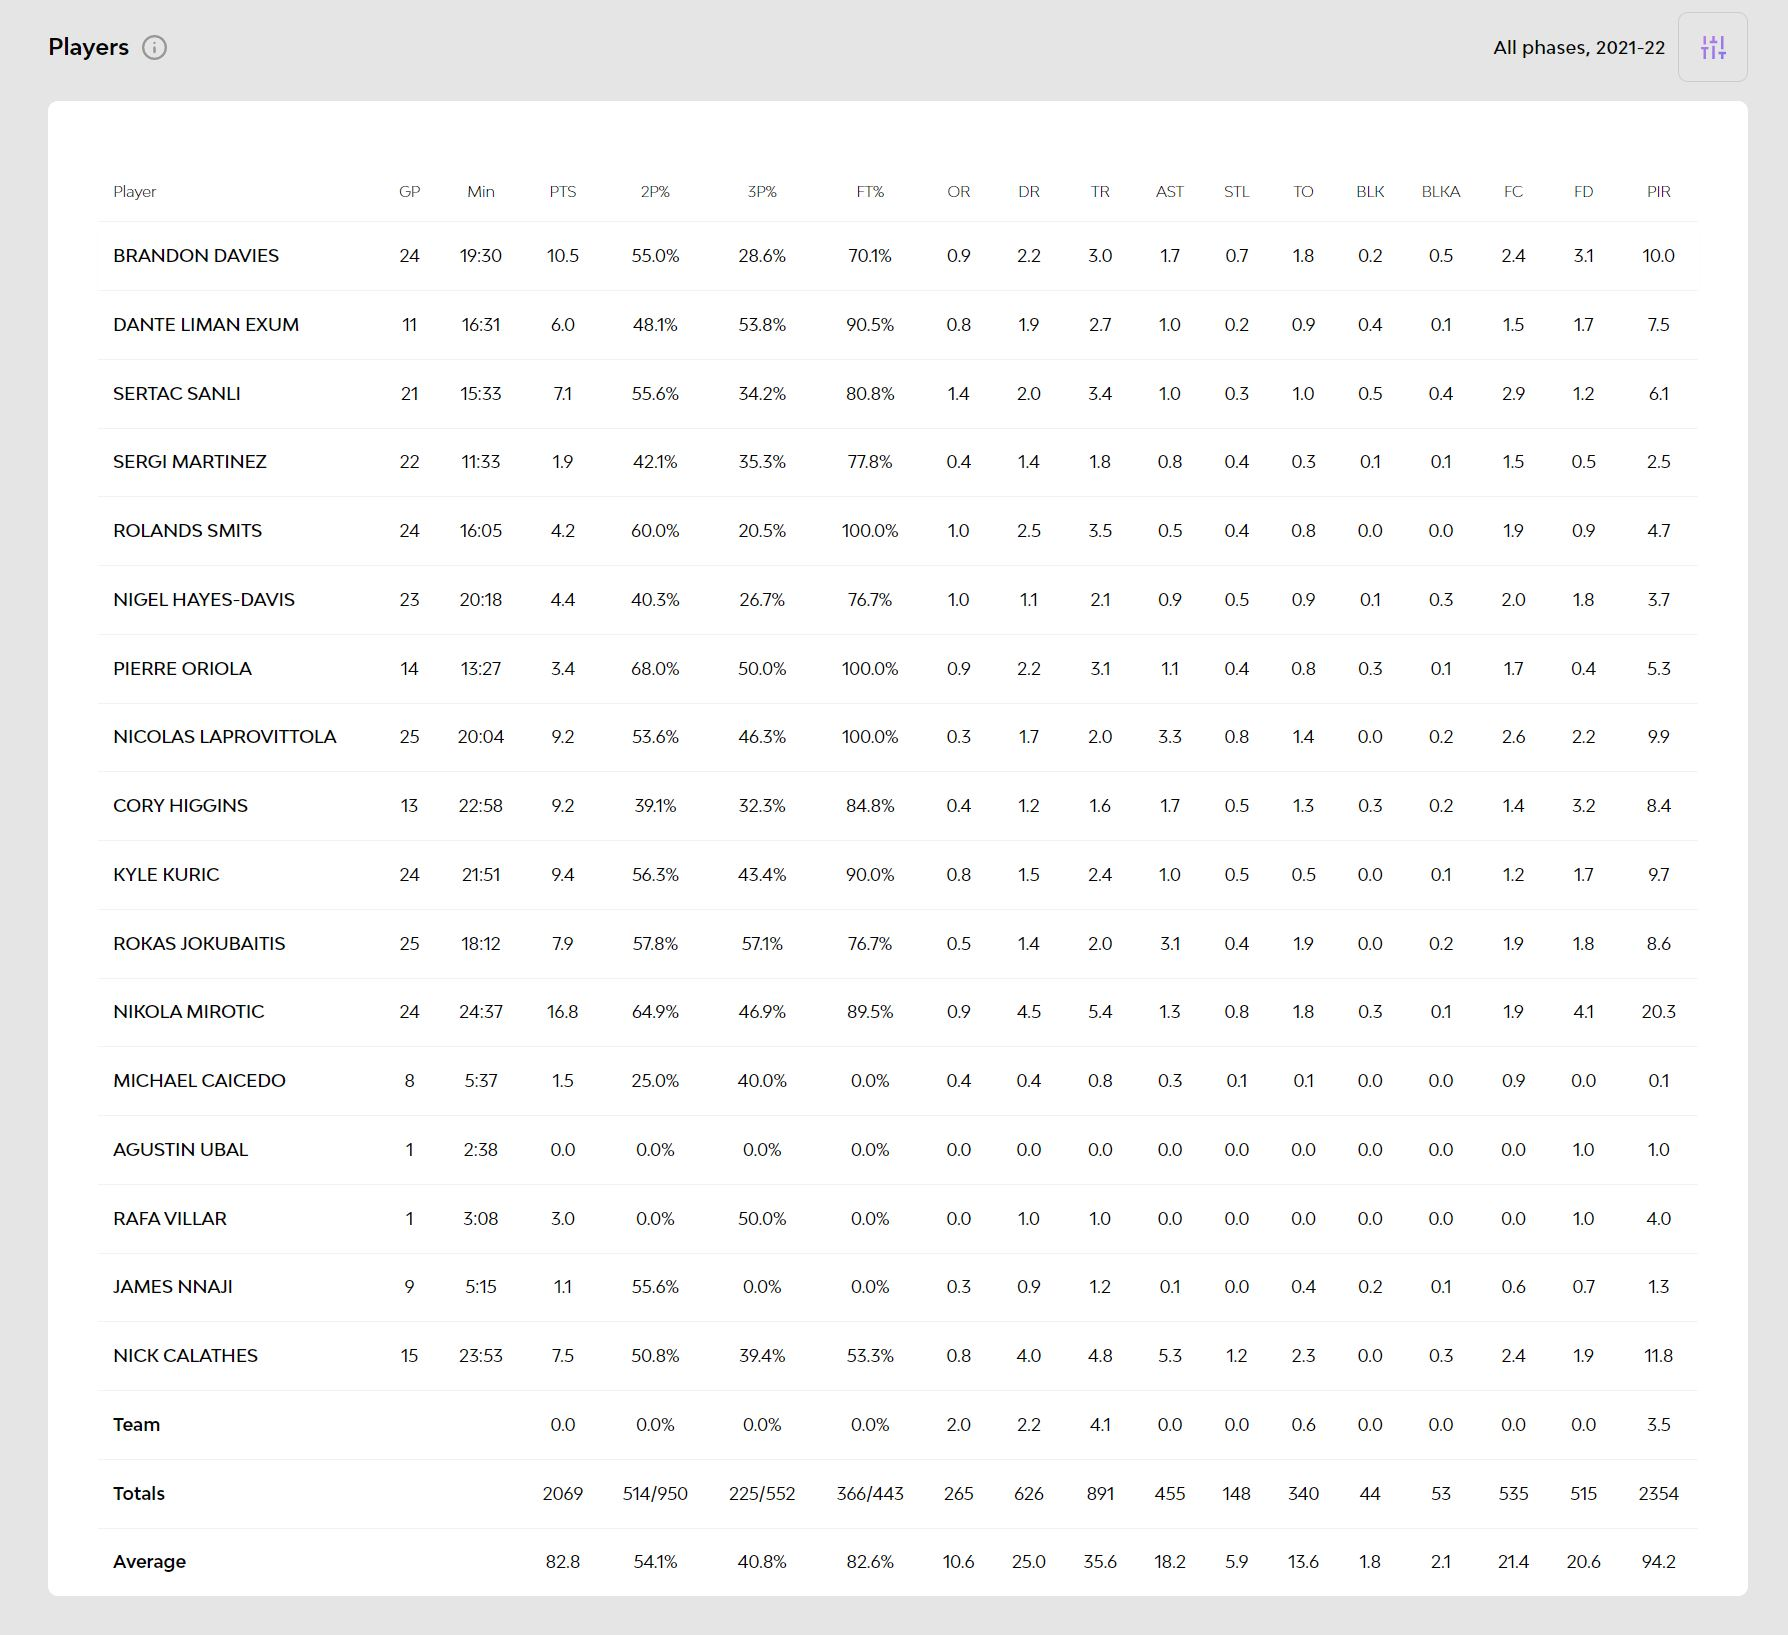
\includegraphics[width=.9\linewidth]{BoxScore2022.jpg}
  \captionof{figure}{Boxscore del partido de la Euroliga de Real Madrid contra FC Barcelona, del 11 de Febrero del 2022}
  \label{fig:BoxScore2022}
\end{minipage}
\end{figure}

\end{document}
